\documentclass[../Results.tex]{subfiles}

\begin{document}
	\cite{emonts2019cold} used sensitive low-surface-brightness observations of Very Large Array (VLA) to trace the cold molecular gas in the inner region of MAMMOTH-1 by detecting the CO (1-0) emission. They found four CO sources which are a few kpcs away from the associated galaxies or groups. This result suggests that the core of the potential well of this Ly$\alpha$ nebula is marked by the cold gas rather than the obscured AGN. Since none of the continuum image (center on 35 GHz and 150 GHz) from VLA nor Atacama Large Millimeter/submillimeter Array (ALMA) shows detectable signal, we use them to give a 3-$\sigma$ upper limit on its continuum emission in radio band, $\rm f_{35,up}=0.050$ mJy, $\rm f_{150,up}=0.066$ mJy. By applying these two upper limits with the data from \citet{arrigoni2018overdensity}, we fit the spectral energy distribution (SED) of BOSS1441 with M82 template from \cite{Silva_1998} in Fig.\ref{SED}. Gray lines represent the SED of radio-quiet galaxies in \citet{harrison2014kiloparsec} with the gray square representing the flux density at 1.4 GHz (rest frame) of these sources. The purple points represent the flux of MRC 1138-262 which is also know as spiderweb galaxy with extreme radio emission at z=2.16 \citep{Nesvadba_2006}. The brown dashed line is the average of SEDs belonging to 1056 radio galaxies (RG) with redshifts in the range of $0.0028-1.7$ \citep{Toba_2019}. All of these SEDs and data have been normalized and shifted to $z=2.31$. M82 template fits extremely well with flux of source-B even including the two upper limits from ALMA and VLA, this evidence suggests that source-B should be a star burst galaxy. In addition, the departure of flux of source-B and M82 template from RG template and flux of spiderweb galaxy indicates that there should be no strong radio emission from source-B due to AGN activity.
	
	\begin{figure}[htp]
		\centering
		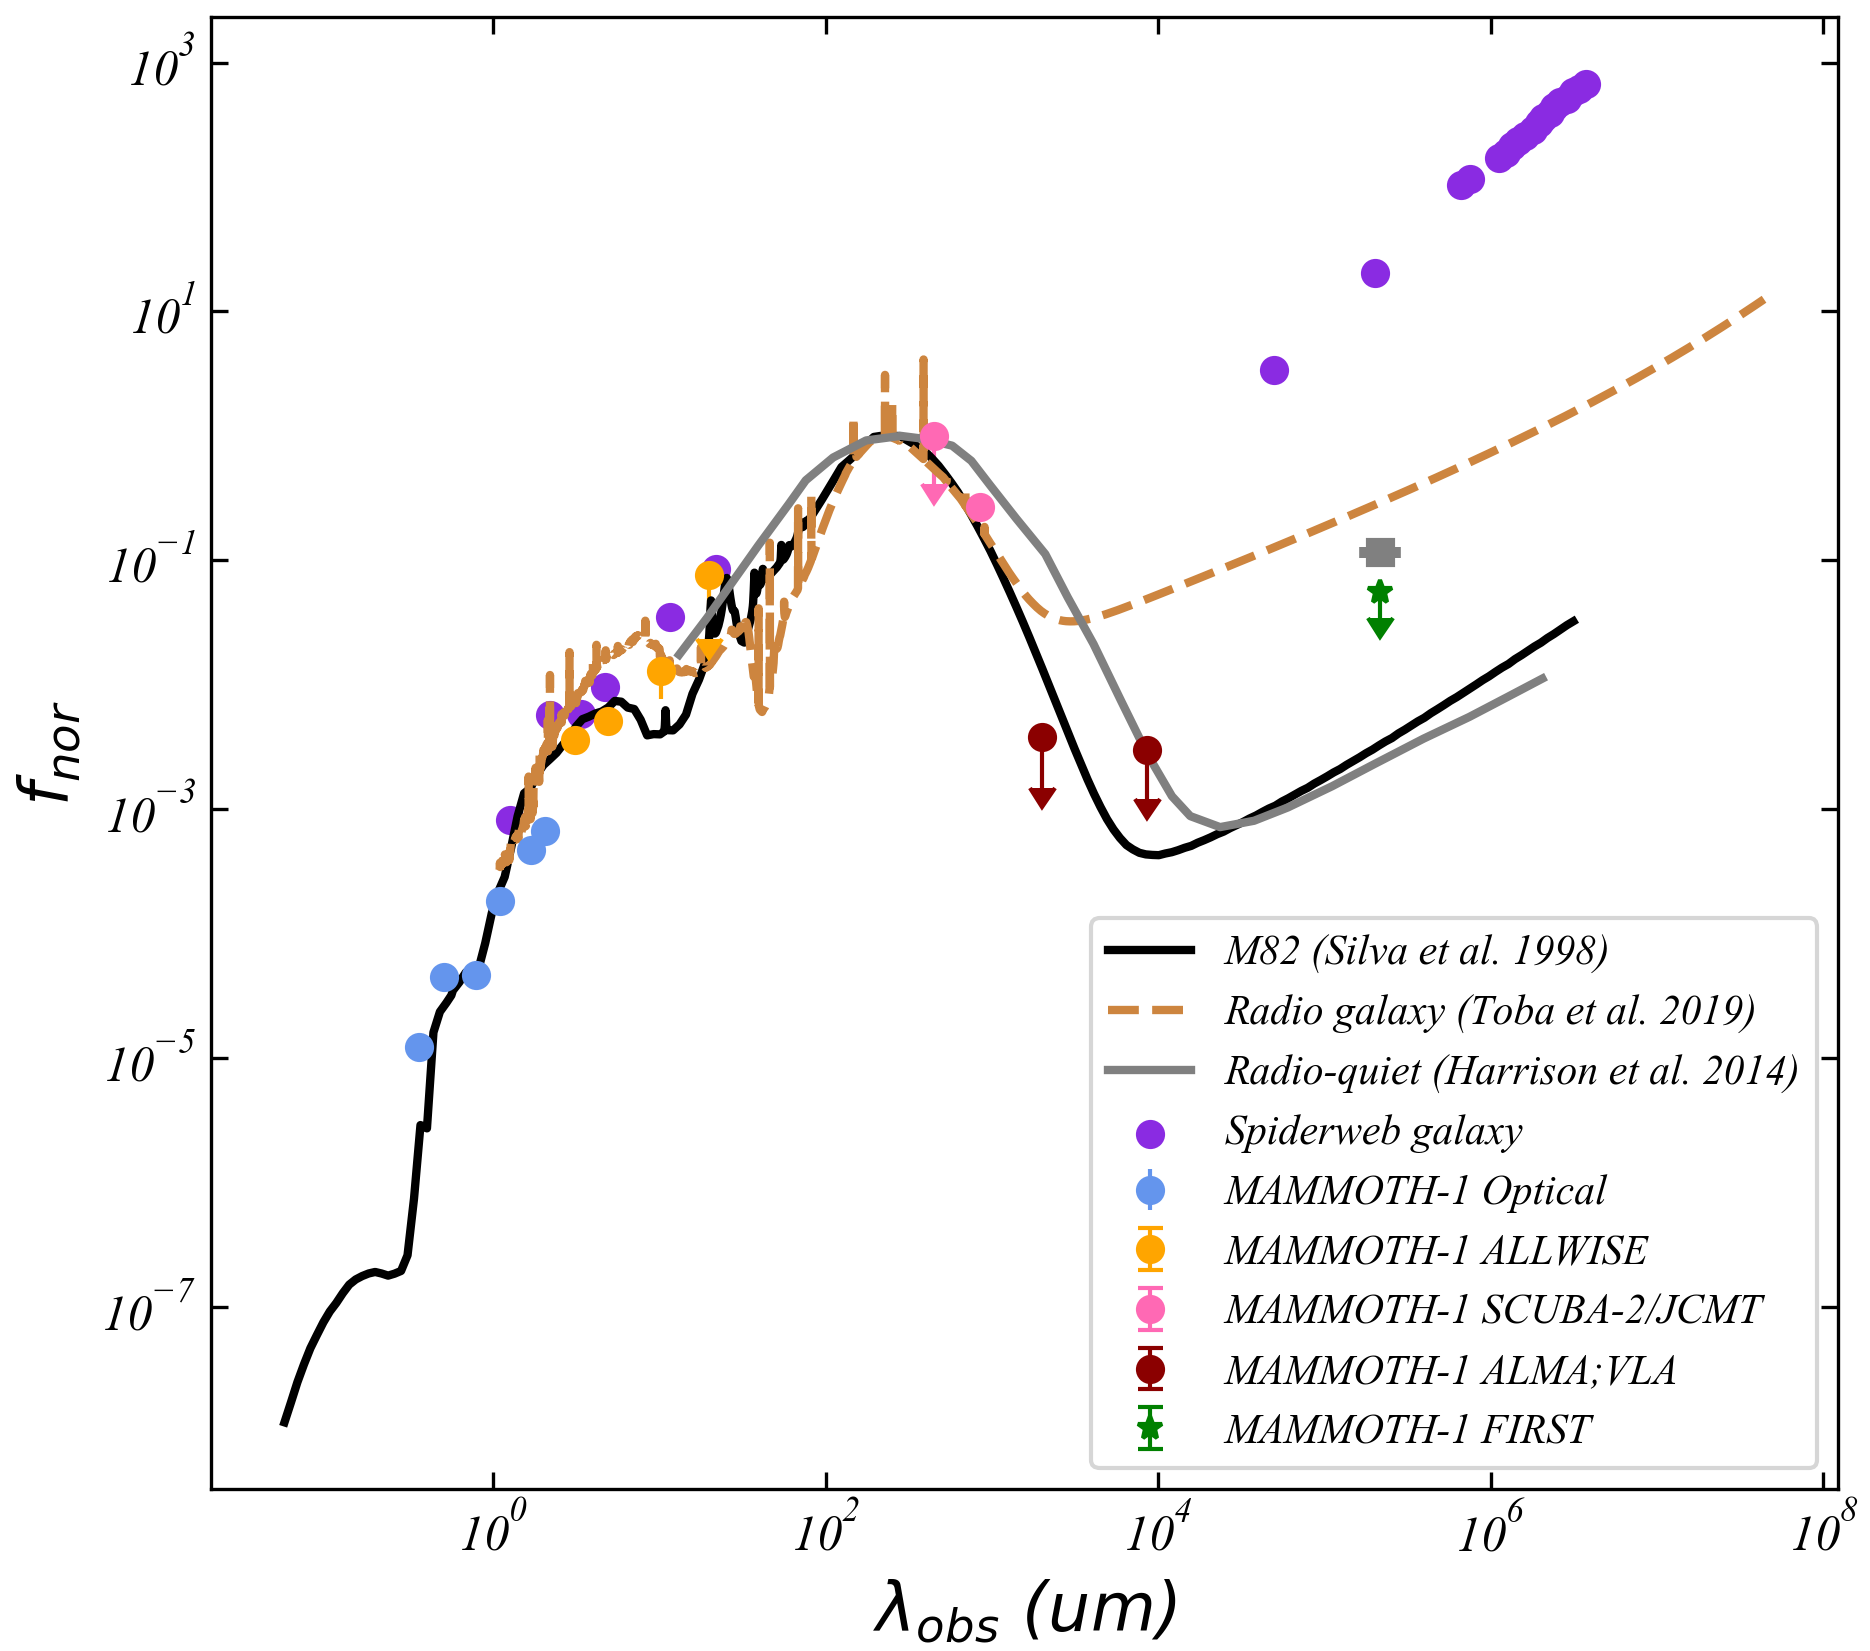
\includegraphics[width=\columnwidth]{figs/SED_fitting}
		\caption{SED for source-B powering ELAN MAMMOTH-1. The data points are from \citet{cai2017discovery} (blue), ALLWISE source catalog, SCUBA-2 data \citep{arrigoni2018overdensity} (magenta), ALMA and VLA continuum images \citep{emonts2019cold} (dark red) and FIRST catalog (green). Gray line represents SED of radio-quiet galaxy while gray square represents flux at 1.4 GHz of "radio-excess" galaxy \citet{harrison2014kiloparsec}. The brown dashed line is the average template of 1056 radio galaxies at redsfhits from 0.0028 to 1.7 \citep{Toba_2019}. All of this data are normalized and shifted to z=2.3.}
		\label{SED}
	\end{figure}
	
	 We calculate the ratio ($\rm q_{IR}$) between the far-infrared flux ($\rm 8-1000 \ \mu m$) and radio flux with the definition given by \cite{ivison2010far}. This ratio is usually used to identify if there is significant radio emission above that expected from their star-formation activity (radio emission results from AGN or other process). The formula is given by:
	\begin{equation}
		\rm q_{IR}=log[\frac{S_{IR}/3.75 \times 10^{12} W \ m^{-2}}{S_{1.4}/W \ m^{-2} Hz^{-1}}]
		\label{q_IR}
	\end{equation}
	where $\rm S_{IR}$ is the rest-frame flux in far-infrared range ($8-1000 \ \rm \mu m $) and $\rm S_{1.4}$ is the flux density at 1.4 GHz in rest frame. The far-infrared luminosity is $\rm L_{IR}=3.2 \times 10^{12}L_{\odot}$ estimated by \citet{arrigoni2018overdensity}. Through setting the luminosity distance to be $\rm D_{L}=18773.8$ Mpc at redshift z=2.3, it is easy to calculate the far-infrared flux $\rm S_{IR}=2.9 \times 10^{-16}\ W \ cm^{-2}$.  Because the D-configuration of VLA doesn't cover $\rm \nu_{obs}=0.42$ GHz (1.4 GHz in rest frame), we adopt $\rm S_{1.4}$=0.01 mJy from M82 SED template. We note here that the constrain of continuum, $\rm f_{150,up}$, is one-order-magnitude lower than that of M82 SED template, therefore the true flux density at $\rm \nu_{rest}=1.4$ GHz is possibly lower than 0.01 mJy. By adopting $\rm S_{1.4}=0.01 mJy$ the low limit of $\rm q_{IR}$ is equal to 1.9. \citet{ivison2010far} and \citet{del2013goods} define "radio-excess" sources as those with $\rm q_{IR} \leqslant 1.8$, this calculation also supports that source-B has no significant radio emission.
	
	Based on these evidences we conclude that source-B is most likely a radio-quiet quasar with no strong radio emission due to AGN activity.
\end{document}